% ************************** Thesis Chapter2 **********************************
\clearpage
\chapter{ทฤษฎี/การวิจัยที่เกี่ยวข้อง}
ในส่วนของงานที่เกี่ยวข้องกับการวิเคราะห์วิดีโอในปัจจุบันนั้นมีความหลากหลายของวิธีในการทำ ผู้วิจัยจึงจำเป็นต้องศึกษาองค์ความรู้และงานวิจัยที่ตรงกับวัตถุประสงค์ของงาน เพื่อศึกษาและเป็นแนวทางในการประยุกต์ใช้สร้าง Video analytics platform ซึ่งหัวข้อที่ผู้วิจัยได้ไปศึกษามา มีดังต่อไปนี้
\begin{enumerate}
	\setlength\itemsep{-0.25em}
	\item การวิเคราะห์ผลวิดีโอ
	\begin{enumerate}	
		\item การตรวจจับวัตถุ
		\item การทำนายตำแหน่งถัดไปของวัตถุ
		\item การระบุตัวตนของบุคคล
		\item การจดจำการกระทำ
	\end{enumerate}
	\setlength\itemsep{-0.25em}
	\item เครื่องมือสำหรับการวิเคราะห์ผลวิดีโอ
	\begin{enumerate}	
		\item Machine learning model
		\item เครื่องมือสำหรับสร้างชุดข้อมูล
	\end{enumerate}
	\item ทฤษฎีที่เกี่ยวข้อง
	\begin{enumerate}	
		\item Optical flow
	\end{enumerate}
\end{enumerate}

\section{การวิเคราะห์ผลวิดีโอ}
ในส่วนของงานวิจัยสิ่งที่เราให้ความสนใจ คือ ข้อมูลการกระทำของมนุษย์แต่ละคนภายในวิดีโอ  ซึ่งเพื่อที่เราจะได้ผลลัพธ์ที่มีประสิทธิภาพออกมาเป็นข้อมูลของสิ่งที่เราสนใจและสามารถนำไปใช้ต่อได้ เราจึงจำเป็นจะต้องใช้การวิเคราะห์ผลวิดีโอเพื่อที่จะสกัดสิ่งที่เราสนใจออกมาจากวิด๊โอ ซึ่งการวิเคราะห์ผลวิดีโอมีหลากหลายกระบวนการในการทำ จะทำทีละขั้นตอน โดยในแต่ละกระบวนการจะมีจุดประสงค์ของการทำและผลลัพธ์หลังการทำที่แตกต่างกัน ในหัวข้อนี้จะมาอธิบายถึงกระบวนการในการวิเคราะห์ผลของวิดิโอและผลลัพธ์ของการทำกระบวนการนั้น

\subsubsection*{2.1.1 การตรวจจับวัตถุ}
การตรวจจับวัตถุเป็นสิ่งที่สำคัญเป็นอันดับต้นๆของการวิเคราะห์ผลของวิดีโอ คือ การตรวจจับวัตถุ กล่าวคือกระบวนการที่ผู้วิจัยจะต้องทำคือระบุสิ่งที่สนใจว่าคืออะไร อยู่ตำแหน่งใด ซึ่งในปัจจุบันการทำการตรวจจับวัตถุมักนำ Machine learning model มาใช้เพื่อช่วยตรวจจับวัตถุที่เราสนใจ ซึ่ง Machine learning model ที่เราเลือกใช้คือ YOLO v3 โดยเหตุผลที่เราเลือกใช้ Machine learning model YOLO v3 จะถูกกล่าวไว้อยู่ในหัวข้อ Machine learning model ในหัวข้อถัดไป
\par
YOLO v3 เป็น Machine learning model ที่ในปัจจุบันนิยมนำมาใช้ตรวจจับวัตถุในงานวิเคราะห์ผลของวิดีโอ เนื่องจากสามารถตรวจจับวัตถุได้แบบเรียลไทม์และมีความแม่นยำ โดยหลักการของ YOLO v3 คือ นำรูปภาพที่ต้องการตรวจจับตำแหน่งของวัตถุผ่าน neural network โดยโครงข่ายจะแบ่งรูปภาพเป็นพื้นที่ และ จะทำนายกรอบสี่เหลี่ยมพร้อมกับทำนายความน่าจะเป็นของแต่ละหมวดหมู่ในแต่ละพื้นที่ สุดท้ายจะเลือกกรอบสี่เหลี่ยมและหมวดหมู่ที่มีค่าคะแนนความน่าจะเป็นมากที่สุด

\subsubsection*{2.1.2 การทำนายตำแหน่งถัดไปของวัตถุ (Tracking)}
การติดตามการเคลื่อนไหวของวัตถุ\textsuperscript{\cite{danelljan2014accurate}} คือระบบที่ใช้สำหรับการติดตามการเคลื่อนไหวของวัตถุที่สนใจที่อยู่ในรูปภาพ 
โดยใช้การคำนวณทางคณิตศาสตร์ และการประมวลผลภาพ (image processing) ทำให้การประมวลผลนั้นเร็วกว่าการใช้โมเดลปัญญาประดิษฐ์ ซึ่งอัลกอริทึมติดตามการเคลื่อนไหวที่นิยมใช้มีสองอัลกอริทึม
คือ correlation filter และ kalman filter ซึ่งหลักการของทั้งสองอัลกอริทึมนั้นจะแตกต่างกันโดยที่ correlation filter นั้นจะใช้พิกเซลของวัตถุในการคำนวณตำแหน่งถัดไปของวัตถุ 
และ kalman filter จะใช้ข้อมูลการเคลื่อนไหวในการคำนวณตำแหน่งถัดไปของวัตถุ ซึ่งจากการศึกษาในบทความ "Object Tracking using Correlation,
Kalman Filterand Fast Means Shift Algorithms"\textsuperscript{\cite{ali2006object}} kalman filter มีประสิทธิภาพที่สูงนั้นจะขึ้นอยู่กับข้อมูลที่ได้จากการวัด (measurement)
และความซับซ้อนในการเคลื่อนไหวของวัตถุ ในขณะที่ correlation นั้นมีประสิทธิภาพที่ด้อยกว่า kalman filter เพียงเล็กน้อยและสามารถติดตามการเคลื่อนไหวที่ซับซ้อนของวัตถุได้ดีกว่า 
(การเคลื่อนไหวที่ซับซ้อนหมายถึง การเคลื่อนไหวที่เกิดการเปลี่ยนทิศทางฉับพลันบ่อย) ผู้วิจัยจึงตัดสินใจเลือกใช้ correlation filter ในงานครั้งนี้
\begin{figure}[!ht]
	\centering
	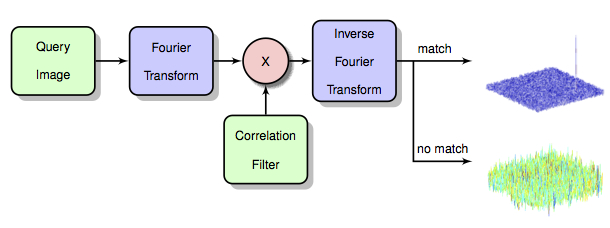
\includegraphics[width=1\textwidth]{chapter2/images/track-concept.png}
		\caption[แนวคิดของระบบติดตามการเคลื่อนไหวของวัตถุ]{แนวคิดของระบบติดตามการเคลื่อนไหวของวัตถุ\textsuperscript{\cite{correlation_filter}}}
    	\label{fig:Track_concept}
\end{figure}

จากรูปที่ \ref{fig:Track_concept} เป็นหลักการในการติดตามการเคลื่อนไหวของวัตถุแบบ correlation filter โดยการนำรูปมาผ่านกระบวนการแปลงฟูรีเยร์ (fourier transform)
และนำมาคูณกับ correlation filter ซึ่งเป็นตัวกรองที่ใช้สำหรับการหาความสัมพันธ์กับวัตถุในภาพ จากนั้นทำการแปลงฟูรีเยร์ผกผัน (inverse fourier transform) 
เพื่อตรวจสอบว่าวัตถุในภาพนั้นอยู่ที่ตำแหน่งใด โดยมีการคำนวณเริ่มจากการหา correlation filter ที่ดีที่สุดโดยใช้วิธีลดผลรวมของข้อผิดพลาดกำลังสองให้น้อยที่สุดดังนี้

\begin{equation}
\epsilon = \left \| \sum_{l = 1}^{d} h^{l} \star f^{l} - g \right \|^2 + \lambda \sum_{l = 1}^{d}\left \| h^{l} \right \|^2
\end{equation}
โดยที่
\begin{conditions}
 \epsilon     	&   ค่าความคลาดเคลื่อน 							\\
 d      		&  จำนวนมิติของผังคุณลักษณะของภาพ  \\   
 h 			&  correlation filter								\\
\star 			&  circular correlation							\\
 f			&  พื้นที่สี่เหลี่ยมของวัตถุที่สนใจที่ได้จากการทำผังคุณลักษณะ	\\
 g			&  ผลลัพธ์ correlation ที่ต้องการของ f					\\
 \lambda   		&  regularization term
\end{conditions}

เมื่อพิจารณาจากรูปภาพเดียวในกรณีที่เวลา ($t$) เท่ากับ 1 จะสามารถจัดรูปสมการด้านบนได้ดังนี้ 

\begin{equation}
H^{l} = \frac{\bar{G}F^{l}}{\sum_{k=1}^{d}\bar{F^{k}}F^{k} + \lambda}
\end{equation}
\begin{equation}
H_{t}^{l} = \frac{A_{t}^{l}}{B_{t}}					
\end{equation}					
\begin{equation}
A_{t}^{l} = (1-\eta )A_{t-1}^{l} + \eta \bar{G_{t}}F_{t}^{l}
\end{equation}
\begin{equation}
B_{t} = (1-\eta )B_{t-1} + \eta \sum_{k=1}^{d}\bar{F_{t}^{k}}F_{t}^{k}
\end{equation}
\clearpage
\noindent
โดยที่
\begin{conditions}
 H 		     	&   correlation filter								\\
 \eta      		&  อัตราการเรียนรู้						 		\\   
 \bar{G} 		&  g ที่ผ่านการทำ complex conjugation					\\
 F			&  พื้นที่สี่เหลี่ยมของวัตถุที่สนใจที่ได้จากการทำผังคุณลักษณะ	\\
 \bar{F}		&   f ที่ผ่านการทำ complex conjugation					\\
 t 	  		&  เวลา
\end{conditions}
จากสมการที่ได้มาจะสามารถทำให้หาตำแหน่งต่อไปของวัตถุที่สนใจได้ด้วยสมการต่อไปนี้
\begin{equation}
y = F^{-1}\left \{ \frac{\sum_{l = 1}^{d} \bar{A^{l}}Z^{l}}{B + \lambda} \right \}
\end{equation}
โดยที่
\begin{conditions}
 y 		     	&   correlation score										\\
 F^{-1}    		&  การแปลงฟูรีเยร์ผกผันแบบไม่ต่อเนื่อง (inverse discrete fourier transform)						\\   	
 \bar{A}^{l} 	&  $A^{l}$ ที่ผ่านการทำ complex conjugation				\\
 Z	 		&  พื้นที่สี่เหลี่ยมของวัตถุที่สนใจที่ได้จากการหาผังคุณลักษณะของภาพใหม่	
\end{conditions}
โดยค่าของ $y$ ที่ได้ออกมาจะทำให้รู้ถึงตำแหน่งของวัตถุที่สนใจได้ ณ ตำแหน่งที่ $y$ มีค่าสูงสุด

\subsubsection*{2.1.3 การระบุตัวตนของบุคคล (ReID)}
ระบบระบุตัวตนของบุคคล\textsuperscript{\cite{luo2019alignedreid++}}\textsuperscript{\cite{zhang2017alignedreid}} คือการระบุตัวตนของบุคคลภายในวิดีโอหรือระหว่างสองภาพ สามารถนำมาประยุกต์ใช้ในด้านของการรักษาความปลอดภัย 
หรือการตามหาบุคคล ซึ่งการระบุตัวตนของบุคคลนั้นเป็นปัญหาที่ท้าทาย เนื่องจากคุณลักษณะทั่วไปของบุคคลในภาพไม่เพียงพอต่อการระบุตัวตนภายในภาพว่าเป็นบุคคลคนเดียวกันได้ ซึ่งวิธีการที่ใช้ในการระบุตัวตนของบุคคลเรียกว่า 
Dynamically Matching Local Information (DMLI) ที่สามารถจัดแนวรายละเอียดข้อมูลของภาพและเพิ่มประสิทธิภาพให้สูงขึ้น 
ถึงแม้ว่า DMLI นั้นจะไม่ใช่วิธีการที่มีประสิทธิภาพสูงสุดแต่มีประสิทธิภาพใกล้เคียงกับโมเดลอื่นๆ แต่ผู้วิจัยสามารถนำวิธีนี้มาประยุกต์เข้ากับงานวิจัยครั้งนี้ได้สะดวกที่สุด จึงนำวิธีการนี้มาใช้สำหรับงานวิจัยครั้งนี้

\begin{figure}[!ht]
	\centering
	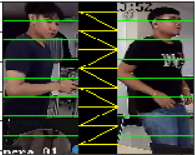
\includegraphics[width=0.3\textwidth]{chapter2/images/alignedreid.png}
		\caption{การแบ่งภาพออกเป็น 8 ส่วนของระบบระบุตัวตนของบุคคล}
    	\label{fig:alignedreid}
\end{figure}

การทำงานของระบบระบุตัวตนของบุคคลจะเริ่มจากการแบ่งภาพออกเป็น 8 ส่วนและนำคุณลักษณะทั่วไปของภาพมาผ่านกระบวนการ normalization เพื่อลดความซ้ำซ้อนของข้อมูล 
แล้วนำมาเปรียบเทียบความแตกต่างของคุณลักษณะทั่วไปของภาพโดยใช้วิธี euclidean distance หลังจากนั้นใช้วิธี DMLI หาความแตกต่างออกมา โดยค่าที่ได้ออกมาจะเรียกว่า aligned distance ถ้าค่าที่ออกมาใกล้เคียงกับศูนย์
จะหมายถึงบุคคลในภาพทั้งสองเป็นบุคคลเดียวกัน โดยใช้การกำหนดเกณฑ์ของ aligned distance สำหรับระบุตัวตนของบุคคลในภาพว่าเป็นบุคคลเดียวกันหรือไม่

โดยชุดข้อมูลที่นำมาใช้สำหรับการทำโมเดลปัญญาประดิษฐ์ได้แก่
\begin{enumerate}
	\item{Market1501 เป็นชุดข้อมูลที่เก็บข้อมูลภาพของบุคคลโดยใช้กล้องจำนวนหกตัว ถ่ายภาพบุคคลที่ด้านหน้าของซุปเปอร์มาร์เก็ตในมหาวิทยาลัย Tsinghua}
	\item{DukeMTMCReID เป็นชุดข้อมูลที่เก็บข้อมูลภาพของบุคคลโดยใช้กล้องจำนวนแปดตัว ถ่ายภาพบุคคลที่วิทยาเขตของมหาวิทยาลัย Duke ซึ่งมีการเก็บภาพมากถึงสองล้านภาพของนักศึกษาสองพันคน }
	\item{CUHK-03 เป็นชุดข้อมูลที่เก็บภาพของบุคคลที่มหาวิทยาลัยที่ฮ่องกง}
	\item{MSMT17 เป็นชุดข้อมูลที่เก็บข้อมูลภาพของบุคคลโดยใช้กล้องจำนวนสิบห้าตัว โดยที่กล้องแต่ละตัวจะไม่ได้ตั้งอยู่สถานที่เดียวกัน และเก็บข้อมูลที่ในวันที่มีสภาพอากาศต่างกัน}
\end{enumerate}

โดยทุกชุดข้อมูลจะใช้โครงสร้าง (architecture) ResNet50 ในการสร้างโมเดลปัญญาประดิษฐ์ และทดสอบด้วยวิธี Global+DMLI คือการนำคุณลักษณะทั่วไปและคุณลักษณะจำเพาะของภาพที่ได้มาจากโมเดลปัญญาประดิษฐ์ นำมาหาค่าระยะความแตกต่าง โดยที่ค่าระยะความแตกต่างของคุณลักษณะทั่วไปสามาหาได้โดยใช้วิธี Euclidean distance และค่าระยะความแตกต่างของคุณลักษณะจำเพาะสามารถหาได้โดยใช้วิธี DMLI และนำมาเทียบกับชุดข้อมูลทดสอบเพื่อคำนวณหาค่า rank1 และ mAP โดยที่ค่า rank1 หมายถึงค่าอัตราร้อยละของความมั่นใจสูงสุดของโมเดลปัญญาประดิษฐ์ที่ทำนายออกมาถูกต้อง 
และค่า mAP คือการหาค่าเฉลี่ยความแม่นยำในแต่ละหมวดหมู่ ซึ่งสามารถดูค่า rank1 และ mAP ของโมเดลปัญญาประดิษฐ์สำหรับการทำระบุตัวตนของบุคคลได้ในหัวข้อที่ \ref{sec:reid_ex}

วิธีการคำนวณของ DMLI ในขั้นตอนการสร้างโมเดลปัญญาประดิษฐ์ของการระบุตัวตนบุคคล
\begin{equation}
d_{i,j} = \frac{e^{\left \| f_{i} - g_{j} \right \|^{2}} - 1}{e^{\left \| f_{i} - g_{j} \right \|^{2}} + 1} \qquad i,j \epsilon 1,2,3,..H
\end{equation}

โดยที่
\begin{conditions}
d		&		เมทริกซ์ของระยะความแตกต่างที่น้อยที่สุดของคุณลักษณะจำเพาะของทั้งสองภาพ			\\
f		&		ค่าคุณลักษณะจำเพาะของรูปภาพที่ 1				\\
g		&		ค่าคุณลักษณะจำเพาะของรูปภาพที่ 2				\\
H		&		จำนวนภาพแนวตั่งที่แบ่งออกมา
\end{conditions}

\begin{equation}
S_{i,j} = \begin{cases}
d_{i,j} & \text{ if } i=1,j=1 \\ 
S_{i-1,j}+d_{i,j} & \text{ if } i\neq 1,j=1 \\ 
S_{i,j-1}+d_{i,j} & \text{ if } i=1,j\neq1 \\ 
min(S_{i-1,j},S_{i,j-1}) & \text{ if } i\neq1,j\neq1 
\end{cases}
\end{equation}

เมื่อทำการคำนวณ $S_{i,j}$ ซึ่งเป็นผลรวมของระยะความแตกต่างที่น้อยที่สุดแล้วตัวสุดท้ายของ $S_{i,j}$ จะเป็นระยะความแตกต่างที่น้อยที่สุดที่ของคุณลักษณะจำเพาะของทั้งสองภาพ แต่ในกรณีที่ทางผู้วิจัยนำมาใช้งานค่า $d_{i,j}$ นั้นจะเป็นค่าที่ได้มาจากการทำ euclidean distance แทน


\subsubsection*{2.1.4 การจดจำการกระทำ}
การจดจำการกระทำ เป็นกระบวนการในการทำนายการกระทำของมนุษย์หรือสิ่งที่สนใจอื่นๆ ที่เกิดการกระทำขึ้นภายในวิดีโอ โดยในหัวข้อนี้จะกล่าวถึงตั้งแต่ขั้นตอนแรกของการทำการจดจำการกระทำซึ่งก็คือ การได้มาซึ่งชุดข้อมูลมีกระบวนการอย่างไร นอกจากนั้นจะกล่าวถึงการนำ Machine learning model มาใช้ในการจดจำการกระทำ และ การวัดผลของ Machine learning model โดยชุดข้อมูลที่ผู้วิจัยได้เลือกนำมาศึกษาจากชุดข้อมูลที่ถูกเป็นที่กล่าวถึงในปัจจุบัน และ มีขนาดของชุดข้อมูลที่ใหญ่ 
\par
จากบทความข้างต้นชุดข้อมูลที่เราได้เลือกนำมาใช้ได้แก่ ชุดข้อมูล Youtube-8M , AVA , Moment in Time โดยแต่ละชุดข้อมูลจะมีความแตกต่างกันในหลายๆด้าน แต่จะมีสิ่งที่แต่ละชุดข้อมูลมีเหมือนกัน คือ เป็นชุดข้อมูลสำหรับการวิเคราะห์ผลวิดีโอที่มีการสนใจการกระทำของมนุษย์ โดยในบทความนี้จะกล่าวถึงความแตกต่างในด้านต่างๆ เช่น เป้าหมายของแต่ละชุดข้อมูล , วิธีการเก็บข้อมูลสำหรับชุดข้อมูล , วิธีการสร้างงคำอธิบาย และ รายละเอียดของชุดข้อมูล โดยจะสรุปข้อมูลของแต่ละชุดข้อมูลด้านล่าง
\begin{enumerate}
%%%%%%%%%%%%%%%%%%%%%%%%%%%%%%%%%%%%%%%%%%%%%%%%%%%%%%%%%%%%%%%%%%%%%%%%%%%%%
	\item \textbf{Youtube-8M}
	\begin{enumerate}
		\setlength\itemsep{-0.25em}
		\item เป้าหมายของชุดข้อมูล :ใช้ทำนายธีมของวิดีโอ
		\item กฏในการรวบรวมข้อมูลดังนี้
		\begin{enumerate}
			\setlength\itemsep{-0.25em}
			\item ทุกๆ หัวข้อต้องเป็นรูปธรรม
			\item ในแต่ละหัวข้อต้องมีจำนวนวิดีโอไม่น้อยกว่า 200 วิดีโอ
			\item ความยาวของวิดีโอต้องอยู่ระหว่าง 120 - 500 วินาที
		\end{enumerate}
		หลังจากได้กฏในการรวบรวมข้อมูลแล้ว ขั้นตอนต่อไปคือการสร้างคำศัพท์ที่ใช้ในการค้นหาข้อมูลวิดีโอจากใน YouTube 
		\item ขั้นตอนในการสร้างคำศัพท์มีดังนี้
		\begin{enumerate}
			\setlength\itemsep{-0.25em}
			\item กำหนด whitelist หัวข้อที่เป็นรูปธรรมมา 25 ชนิด เช่น เกมส์ เป็นต้น
			\item กำหนด blacklist หัวข้อที่คิดว่าไม่เป็นรูปธรรมไว้ เช่น software เป็นต้น
			\item รวบรวมหัวข้อที่มีอยู่ใน whitelist อย่างน้อย 1 หัวข้อ และต้องไม่มีอยู่ใน blacklist ซึ่งจะทำให้ได้หัวข้อที่ต้องการมาประมาณ 50,000 หัวข้อ
			\item จากนั้นใช้ผู้ประเมินจำนวน 3 คน ในการคัดหัวข้อที่คิดว่าเป็นรูปธรรม และสามารถจดจำหรือเข้าใจได้ง่ายโดยไม่ต้องเชี่ยวชาญในด้านนั้นๆ ซึ่งผู้ประเมิน ก็จะมีคำถามว่า “ มันยากขนาดไหนถึงจะระบุได้ว่ามีหัวข้อดังกล่าวอยู่ในรูปหรือวิดีโอ โดยใช้เพียงแค่การมองรูปภาพเท่านั้น? ” โดยแบ่งเป็นระดับดังนี้
			\begin{enumerate}
				\setlength\itemsep{-0.25em}
				\item บุคคลทั่วไปสามารถเข้าใจได้
				\item บุคคลทั่วไปที่ผ่านการอ่านบทความที่เกี่ยวข้องมาแล้วสามารถเข้าใจได้
				\item ต้องเชี่ยญในด้านใดซักด้านจึงจะเข้าใจได้
				\item เป็นไปไม่ได้ ถ้าไม่มีความรู้ที่ไม่ได้เป็นรูปธรรม
				\item ไม่เป็นรูปธรรม
			\end{enumerate}
			\item หลังจากคำถามข้างบนและการให้คะแนน จะทำการเก็บไว้เฉพาะหัวข้อที่มีคะแนนเฉลี่ยมากที่สุดอยู่ที่ประมาณ 2.5 คะแนนเท่านั้น
			\item ทำให้สุดท้ายเหลือเพียงประมาณ 10,000 หัวข้อที่สามารถใช้ได้
			\item หลังจากได้หัวข้อที่คิดว่าเป็นรูปธรรมแล้วก็นำไปค้นหาและรวบรวมด้วย YouTube annotation system โดยมีขั้นตอนดังนี้										\begin{enumerate}
				\setlength\itemsep{-0.25em}
				\item สุ่มเลือกวิดีโอมา 10 ล้านวิดีโอ พร้อมกับหัวข้อของวิดีโอ โดยใช้กฏที่กำหนดไว้ เอาหัวข้อที่มีจำนวนวิดีโอน้อยกว่า 200 วิดีโอออก
				\item ทำให้เหลือจำนวนวิดีโออยู่ 8,264,650 วิดีโอ
				\item แยกออกเป็น 3 ส่วน Train set, Validate set และ Test set ในอัตราส่วน 70:20:10 ตามลำดับ
			\end{enumerate}
		\end{enumerate}
	\end{enumerate}
%%%%%%%%%%%%%%%%%%%%%%%%%%%%%%%%%%%%%%%%%%%%%%%%%%%%%%%%%%%%%%%%%%%%%%%%%%%%%
	\item \textbf{AVA}
	\begin{enumerate}
		\setlength\itemsep{-0.25em}
		\item เป้าหมายของชุดข้อมูล : สนใจการกระทำของมนุษย์เป็นศูนย์กลาง
		\item ขั้นตอนการเก็บข้อมูลสำหรับการทำชุดข้อมูลมีขั้นตอนการทำ 5 ขั้น คือ
	\begin{enumerate}
%
		\item การสร้างคำศัพท์การกระทำ จะมีหลัก 3 ข้อในการรวบรวมคำศัพท์ คือ
		\begin{enumerate}
			\item เก็บรวบรวมคำศัพท์ทั่วไปที่เกิดขึ้นในชีวิตประจำวัน
			\item จะต้องมีเอกลักษณ์ สามาถเห็นได้ชัดเจน เช่น การถือของ
			\item กำหนดรูปแบบของคำศัพท์ขึ้นมาและใช้ความรู้จากชุดข้อมูลอื่น ในการทำให้ได้หมวดหมู่ของการกระทำของมนุษย์ที่ครอบคลุมของชุดข้อมูล AVA
		\end{enumerate}
		\setlength\itemsep{-0.25em}
%
		\item  หนังและส่วนที่เลือกมาใช้วิดิโอที่ใช้ทำชุดข้อมูล AVA ทั้งหมดจะถูกนำมากจาก youtube โดยเริ่มจากการรวบรวมเอารายชื่อของนักแสดงที่มีชื่อเสียง ซึ่งจะมีความหลากหลายของเชื้อชาติรวมกันอยู่ ซึ่งวิดิโอที่ถูกคัดเลือกจะมีเกณฑ์ดังนี้ คือ
			\begin{enumerate}
				\item วิดิโอต้องอยู่ในหมวด หนัง และ ละครโทรทัศน์
				\item จะต้องมีความยาวมากกว่า 30 นาที
				\item อัพโหลดเป็นเวลาอย่างน้อย 1 ปี
				\item มียอดวิวคนดูมากกว่า 1000 วิว
				\item ละเว้นวิดิโอบางประเภท เช่น ขาว-ดำ , ความละเอียดต่ำ , การ์ตูน , วิดิโอเกม
			\end{enumerate}
%
		\item  การตีกรอบบุคคลที่อยู่ภายในภาพ ประกอบด้วย 2 ขั้นตอน
			\begin{enumerate}
				\item สร้างกรอบสี่เหลี่ยม โดยใช้โมเดล Faster R-CNN สำหรับการตรวจจับมนุษย์
				\item นำมนุษย์มาใช้ในการตรวจสอบและแก้ไขกรอบสี่เหลี่ยมที่พลาดไป หรือ ตรวจจับผิด
			\end{enumerate}	
		\item  การเชื่อมของบุคคลในช่วงระยะเวลาสั้นๆของเฟรม 
\\
ทำการเชื่อมกรอบสี่เหลี่ยมที่อยู่ในช่วงเวลาเดียวกัน ซึ่งใช้วิธีการ track โดยยึดมนุษย์เป็นศูนย์กลาง ซึ่งจะนำมาคำนวณความใกล้เคียงกันโดยการจับคู่กรอบสี่เหลี่ยม และ ใช้ person embedding จากนั้นจะใช้ Hungarian algorithm ในการหาตัวเลือกที่ดีที่สุด

%
		\item การสร้างคำอธิบาย
\\
		การสร้างคำอธิบายของการกระทำจะถูกสร้างจากเหล่าคนที่เป็นผู้สร้างคำอธิบาย ซึ่งจะใช้หน้าต่างโปรแกรมสำหรับช่วยเหลือในการสร้างซึ่งใน 1 กรอบสี่เหลี่ยม สามารถมีคำอธิบายของการกระทำได้สูงสุดถึง 7 labels นอกจากนั้นสามารถตั้งสถานะบล็อกเนื้อหาที่ไม่เหมาะสม หรือ กรอบสี่เหลี่ยมที่ผิดพลาดได้อีกด้วย ในทางปฎิบัติจะสังเกตได้ว่ามันมีโอกาศผิดอย่างหลีกเลี่ยงไม่ได้ เมื่อต้องได้รับคำสั่งให้หาคำอธิบายของการกระทำที่ถูกต้องจาก 80 หมวดหมู่ จึงแบ่งขั้นตอนออกเป็น 2 ขั้นตอน คือ
		\begin{enumerate}
			\item ข้อเสนอของการกระทำสอบถามเหล่าผู้สร้างคำอธิบาย เพื่อสร้างข้อเสนอสำหรับคำอธิบายของการกระทำจากนั้นจับกลุ่มเข้าด้วยกัน ซึ่งจะทำให้มีโอกาสถูกต้องมากกว่าเป็นข้อเสนอแยกเดี่ยว
			\setlength\itemsep{-0.25em}
			\item ผู้ตรวจสอบข้อเสนอจะตรวจสอบข้อเสนอที่ได้จากขั้นตอนแรก ซึ่งในแต่ละวิดิโอคลิปจะใช้มนุษย์ในการตรวจสอบ 3 คน เมื่อคำอธิบายของการกระทำ ถูกตรวจสอบด้วยผู้ตรวจสอบข้อเสนออย่างน้อย 2 คน คำอธิบายของการกระทำนั้นจะถูกยึดเป็นคำอธิบายหลัก
		\end{enumerate}
	\end{enumerate}
	\end{enumerate}
%%%%%%%%%%%%%%%%%%%%%%%%%%%%%%%%%%%%%%%%%%%%%%%%%%%%%%%%%%%%%%%%%%%%%%%%%%%%
	\item \textbf{Moment in Time}
	\begin{enumerate}
		\setlength\itemsep{-0.25em}
		\item เป้าหมายของชุดข้อมูล : สนใจการกระทำทุกการกระทำในวิดิโอ เช่น การกระทำของ คน สัตว์ สิ่งของ และ ปรากฎการณ์ธรรมชาติ 
		\item วิธีการเก็บรวบรวมข้อมูล : 
	\begin{enumerate}
	\item เริ่มจากการรวบรวมคำ (verb) ที่มีการใช้อยู่ทั่วไปในชีวิตประจำวันมา 4,500 คำจาก VerbNet จากนั้นนำมาแบ่งกลุ่มคำ(verb) ที่มีความหมายใกล้เคียงกันโดยใช้ features จาก Propbank และ FrameNet โดยเก็บข้อมูลเป็นแบบ binary feature vector ซึ่งถ้าคำ (verb) ไหนมีความเกี่ยวข้องกับ feature ก็จะให้ค่าเป็น 1 ถ้าไม่เกี่ยวข้องกันจะให้ค่าเป็น 0 จากนั้นจึงใช้วิธี k-means clustering ในการแบ่งกลุ่ม เมื่อแบ่งกลุ่มแล้วจากนั้นจะเลือกคำ (verb) จากในแต่ละกลุ่มนั้น โดยคำ (verb) ที่เลือกมานั้นจะเป็นที่ใช้บ่อยที่สุดในกลุ่มนั้น และลบคำ (verb) นั้นออกจากกลุ่มทั้งหมด (คำ ๆ หนึ่งสามารถอยู่ได้หลายกลุ่ม) จากนั้นจะทำกระบวนการนี่ไปเรื่อย ๆ แต่คำ (verb) ที่เลือกมาจะต้องไม่มีความหมายคลุมเครือ ไม่สามารถมองเห็นหรือได้ยินได้ และต้องไม่มีความหมายเหมือนกับคำ (verb) ที่เคยเลือกมาก่อน จนสุดท้ายแล้วได้ออกมาที่ 339 class
	\item ต่อมาทำการหาชุดข้อมูลวิดีโอโดยจะตัดออกมาเพียง 3 วินาทีที่เกี่ยวข้องกับคำ (verb) ใน 339 class ที่เลือกมา จากวิดีโอ แหล่งต่างกัน 10 แหล่ง การตัดวิดีโอนั้นจะไม่ใช้พวก Video2Gif (โมเดลที่ระบุตำแหน่งของสิ่งที่น่าสนใจในวิดีโอ) เพราะจะทำให้เกิด bias ขึ้นจะเกิดขึ้นตอนสร้างโมเดลจากนั้นจะทำการส่งข้อมูลของคำ (verb) และวิดีโอที่ตัดไปยัง Amazon Mechanical Turk (AMT หรือตลาดแรงงาน) เพื่อทำการ label โดยพนักงานแต่ละคนของ AMT จะได้ 64 วิดีโอซึ่งเกี่ยวข้องกับคำ (verb) หนึ่ง และอีก 10 วิดีโอที่มีการทำ label อยู่แล้ว โดยวิดีโอที่มีการทำ label ถ้ามีพนักงานของ AMT ตอบเหมือนกันกับที่ทำ label ไว้เกิน 90\% ถึงจะนำเข้าไปรวมกับชุดข้อมูลส่วนอีก 64 วิดีโอถ้าเป็นของ training set จะต้องผ่านพนักงานของ AMT อย่างน้อย 3 ครั้ง และต้อง label เหมือนกัน 75\% ขึ้นไปถึงจะถือว่าเป็น label ที่ถูกต้อง ถ้าเป็นของ validation และ test set จะต้องผ่านพนักงานของ AMT อย่างน้อย 4 ครั้ง และต้อง label เหมือนกัน 85\% ขึ้นไป ที่ไม่ตั่งเกณฑ์ไว้ที่ 100\% เพราะจะทำให้วิดีโอนั้นยากเกินไปที่จะทำให้สามารถจำการกระทำได้	
\end{enumerate}
\end{enumerate}
%%%%%%%%%%%%%%%%%%%%%%%%%%%%%%%%%%%%%%%%%%%%%%%%%%%%%%%%%%%%%%%%%%%%%%%%%%%%
\end{enumerate}		

\clearpage
\section{เครื่องมือสำหรับการวิเคราะห์ผลวิดีโอ}
\subsection{Machine learning model}
\subsection{เครื่องมือสำหรับสร้างชุดข้อมูล}
จากการค้นคว้าหาเครื่องมือในการสร้างคำกำกับข้อมูลเพื่อใช้เป็นแนวทางในการออกเครื่องมือสำหรับกำกับข้อมูลด้วยปัญญาประดิษฐ์ พบเครื่องมือที่เปิดให้ใช้ง่นสาธารณะ (open source) 2 เครื่องมือ 
คือ DarkLabel และ OpenLabeling โดยสรุปข้อสำคัญได้ดังนี้ 
\subsubsection*{โปรแกรม DarkLabel}
เป็นโปรแกรมที่ช่วยในการทำนายคำกำกับและบันทึกในรูปแบบต่างๆ รองรับข้อมูลป้อนเข้าในรูปแบบไฟล์วิดีโอ avi, mpg หรือกลุ่มรูปภาพ มีขั้นตอนการสร้างคำกำกับดังนี้ 
\begin{enumerate}
	\setlength\itemsep{-0.25em}
	\item สร้างกรอบสี่เหลี่ยมครอบบริเวณวัตถุที่สนใจโดยใช้มนุษย์เป็นคนสร้าง
	\item กดปุ่ม Next และ Predict อย่างต่อเนื่อง เพื่อทำนายตำแหน่งต่อไปของกรอบสี่เหลี่ยมในเฟรมถัดๆไป จนกระทั่งการเกิดข้อผิดพลาด
	\item ลบกรอบสี่เหลี่ยมที่พลาด และเริ่มทำขั้นตอนที่ 1 ใหม่ อีกครั้งจนครบทุกเฟรมในวิดีโอ
\end{enumerate}
หลังจากที่ผู้วิจัยได้ทดลองใช้โปรแกรม DarkLabel พบว่า เป็นโปรแกรมที่การทำงานส่วนใหญ่เป็นการสร้างคำกำกับแบบใช้มนุษย์เป็นคนทำด้วยตัวเอง ซึ่งทำให้ใช้เวลาในการทำนาน

\begin{figure}[!ht]
	\centering
	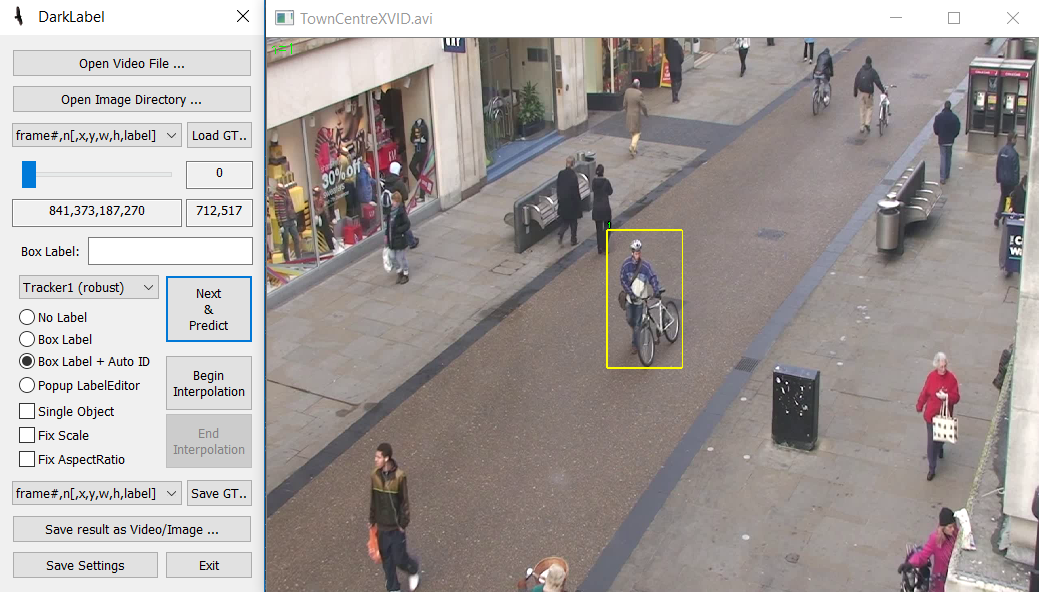
\includegraphics[width=0.7\textwidth]{chapter2/images/darklabel.png}
		\caption{UI ของโปรแกรม DarkLabel}
    	\label{fig:darklabel}
\end{figure}
\clearpage

\subsubsection*{โปรแกรม OpenLabeling}
เป็นโปรแกรมที่ช่วยในการทำนายคำกำกับ โดยโปรแกรมจะมีการทำงานอยู่ 2 รูปแบบการทำงาน คือแบบทำด้วยตัวเอง (Mode Manual) และแบบอัตโนมัติ (Mode Auto) ซึ่งมีการทำงานแยกจากกันอย่างชัดเจน 

\begin{enumerate}
	\setlength\itemsep{-0.25em}
	\item การทำงานแบบอัตโนมัติ 
	\\ หลังจากป้อนวิดีโอเข้าไปในโปรแกรมแล้วมีขั้นตอนการสร้างคำกำกับดังนี้ 
   	\begin{enumerate}
	\setlength\itemsep{-0.25em}
		\item โปรแกรมจะทำงานอัตโนมัติ โดยใช้โมเดลปัญญาประดิษฐ์ในการทำนายคีย์เฟรม (keyframe) 
		และทำนายตำแหน่งต่อไปของกรอบสี่เหลี่ยมในเฟรมถัดไปด้วยอัลกอริทึมที่ใช้การคำนวณคณิตศาสตร์และการประมวลผลภาพ (image processing) ในภาพที่เหลือ ผลลัพธ์ที่ได้คือรูปภาพและไฟล์ข้อมูลคำกำกับ
 	\end{enumerate}
	\item การทำงานแบบทำด้วยตัวเอง 
	\\ หลังจากป้อนวิดีโอเข้าไปในโปรแกรมแล้วมีขั้นตอนการสร้างคำกำกับดังนี้ 
	\begin{enumerate}
	\setlength\itemsep{-0.25em}
		\item สร้างกรอบสี่เหลี่ยมขึ้นมาโดยใช้มนุษย์เป็นคนสร้าง
		\item กดปุ่มเพื่อทำนายตำแหน่งต่อไปของกรอบสี่เหลี่ยมในเฟรมถัดไป จนกระทั่งเกิดข้อผิดพลาด
		\item ลบกรอบสี่เหลี่ยมที่พลาด และเริ่มทำขั้นตอนที่ 1 อีกครั้งจนครบทุกเฟรมในวิดีโอ
 	\end{enumerate}
 \end{enumerate}
หลังจากที่ได้ทดลองใช้โปรแกรม OpenLabeling ทั้ง 2 รูปแบบการทำงานแล้วพบว่า การทำงานแบบอัตโนมัติไม่สามารถปรับแก้ไขสิ่งใดในระหว่างกระบวนการนั้น 
ทำให้หากเกิดกรณีที่โมเดลทำนายกรอบสี่เหลี่ยมพลาดหรือเกินมา จะไม่สามารถแก้ไขได้ และการทำงานแบบทำด้วยตัวเองไม่มีระบบตรวจสอบกรอบสี่เหลี่ยม ทำให้ผู้ใช้งานจะต้องสร้างกรอบสี่เหลี่ยมขึ้นมาเอง

\begin{figure}[!ht]
	\centering
	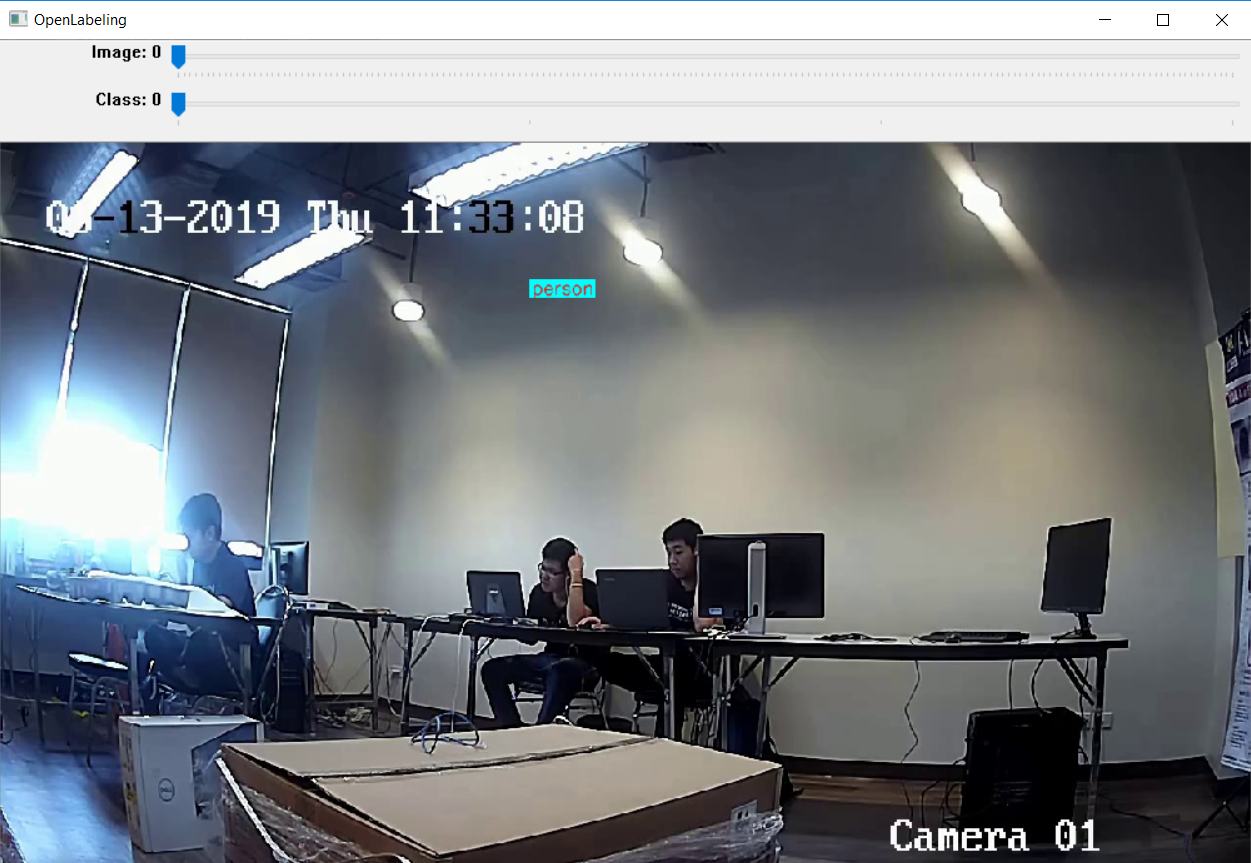
\includegraphics[width=0.7\textwidth]{chapter2/images/openlabel.png}
		\caption{UI ของโปรแกรม OpenLabeling}
    	\label{fig:openlabel}
\end{figure}




\clearpage
%\section{ชุดข้อมูล}
%\subsubsection*{Youtube-8M}
YouTube-8M คือชุดข้อมูลวิดีโอที่เป็น multi-label ที่มีจำนวนวิดีโอเยอะที่สุด ซึ่งมีจำนวนมากถึง 8 ล้านวิดีโอ(ในปี 2016) โดยมีจุดมุ่งหมายหลักในการอธิบายธีมหลักของวิดีโอด้วยคำสั้นๆ เช่น ถ้าวิดีโอนั้นเป็นวิดีโอที่มี มนุษย์กำลังปั่นจักรยานบนถนนดินกับหน้าผา ชุดข้อมูลนี้จะอธิบายวิดีโอนี้ว่า mountain biking ซึ่งทำให้ YouTube-8M แตกต่างจากชุดข้อมูลวิดีโออื่นๆส่วนใหญ่ที่จะเน้น action หรือ activity ของมนุษย์ ซึ่งข้อมูลเชิงสถิติจะเป็นดังตารางที่ 1

\begin{figure}[!ht]
	\centering
	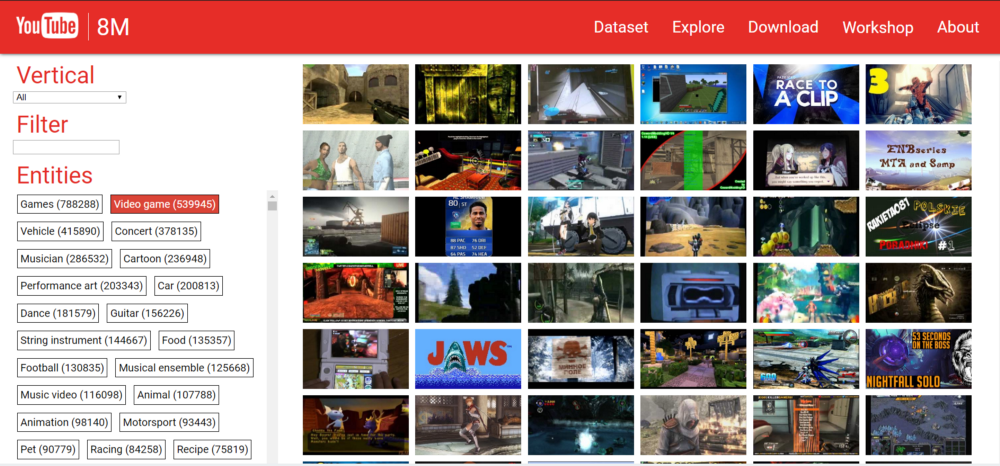
\includegraphics[width=1\textwidth]{chapter2/images/youtube-8m.png}
		\caption{ตัวอย่าง catagories ต่างๆของ YouTube-8M}
    	\label{fig:youtube-8m}
\end{figure}

\begin{table}[!ht]
\begin{tabular}{|c|c|c|c|c|}
		\hline
		{จำนวนวิดีโอ}&{ความยาวโดยรวมของวิดีโอ(ชม.)}&{จำนวนคลาสของวิดีโอ}&{ความยาวเฉลี่ยของแต่ละวิดีโอ(วินาที)}&{(จำนวนคลาสเฉลี่ยในแต่ละวิดีโอ)}\\
		\hline
		8,264,650			& ~500,000		& 4800		& 229.6		& 1.8											\\
		\hline
	\end{tabular}
	\caption{ข้อมูลเชิงสถิติของ YouTube-8M}
	\label{tab: ข้อมูลเชิงสถิติของ YouTube-8M}
\end{table}

\subsubsection*{1. วิธีการรวบรวมข้อมูล}
การเก็บข้อมูลของ YouTube-8M นั้นใช้เครื่องมือที่ชื่อว่า YouTube annotation system ในการเก็บรวบรวมข้อมูลโดยอาศัยผังความรู้(knowledge graph)ของ Google ในการค้นหาและรวบรวมข้อมูลในฐานข้อมูลของ YouTube
\begin{enumerate}
	\setlength\itemsep{-0.25em}
	\item กฏในการรวบรวมข้อมูลดังนี้
	\begin{enumerate}
		\setlength\itemsep{-0.25em}
		\item ทุกๆ หัวข้อต้องเป็นรูปธรรม
		\item ในแต่ละหัวข้อต้องมีจำนวนวิดีโอไม่น้อยกว่า 200 วิดีโอ
		\item ความยาวของวิดีโอต้องอยู่ระหว่าง 120 - 500 วินาที
	\end{enumerate}
หลังจากได้กฏในการรวบรวมข้อมูลแล้ว ขั้นตอนต่อไปคือการสร้างคำศัพท์(vocabulary)ที่ใช้ในการค้นหาข้อมูลวิดีโอจากใน YouTube 
	\item ขั้นตอนในการสร้างคำศัพท์มีดังนี้
	\begin{enumerate}
		\setlength\itemsep{-0.25em}
		\item กำหนด whitelist หัวข้อที่เป็นรูปธรรมมา 25 ชนิด เช่น game เป็นต้น
		\item กำหนด blacklist หัวข้อที่คิดว่าไม่เป็นรูปธรรมไว้ เช่น software เป็นต้น
		\item รวบรวมหัวข้อที่มีอยู่ใน whitelist อย่างน้อย 1 หัวข้อ และต้องไม่มีอยู่ใน blacklist ซึ่งจะทำให้ได้หัวข้อที่ต้องการมาประมาณ 50,000 หัวข้อ
		\item จากนั้นใช้ผู้ประเมินจำนวน 3 คน ในการคัดหัวข้อที่คิดว่าเป็นรูปธรรม และสามารถจดจำหรือเข้าใจได้ง่ายโดยไม่ต้องเชี่ยวชาญในด้านนั้นๆ ซึ่งผู้ประเมิน ก็จะมีคำถามว่า “ มันยากขนาดไหนถึงจะระบุได้ว่ามีหัวข้อดังกล่าวอยู่ในรูปหรือวิดีโอ โดยใช้เพียงแค่การมองรูปภาพเท่านั้น? ” โดยแบ่งเป็นระดับดังนี้
		\begin{enumerate}
			\setlength\itemsep{-0.25em}
			\item บุคคลทั่วไปสามารถเข้าใจได้
			\item บุคคลทั่วไปที่ผ่านการอ่านบทความที่เกี่ยวข้องมาแล้วสามารถเข้าใจได้
			\item ต้องเชี่ยญในด้านใดซักด้านจึงจะเข้าใจได้
			\item เป็นไปไม่ได้ ถ้าไม่มีความรู้ที่ไม่ได้เป็นรูปธรรม
			\item ไม่เป็นรูปธรรม
		\end{enumerate}
		\item หลังจากคำถามข้างบนและการให้คะแนน จะทำการเก็บไว้เฉพาะหัวข้อที่มีคะแนนเฉลี่ยมากที่สุดอยู่ที่ประมาณ 2.5 คะแนนเท่านั้น
		\item ทำให้สุดท้ายเหลือเพียงประมาณ 10,000 หัวข้อที่สามารถใช้ได้
		\item หลังจากได้หัวข้อที่คิดว่าเป็นรูปธรรมแล้วก็นำไปค้นหาและรวบรวมด้วย YouTube annotation system โดยมีขั้นตอนดังนี้
		\begin{enumerate}
			\setlength\itemsep{-0.25em}
			\item สุ่มเลือกวิดีโอมา 10 ล้านวิดีโอ พร้อมกับหัวข้อของวิดีโอ โดยใช้กฏที่กำหนดไว้ เอาหัวข้อที่มีจำนวนวิดีโอน้อยกว่า 200 วิดีโอออก
			\item ทำให้เหลือจำนวนวิดีโออยู่ 8,264,650 วิดีโอ
			\item แยกออกเป็น 3 ส่วน Train set, Validate set และ Test set ในอัตราส่วน 70:20:10 ตามลำดับ
		\end{enumerate}
	\end{enumerate}
\end{enumerate}

เนื่องจากชุดข้อมูลนี้มีขนาดมากกว่า 100 Terabytes และมีความยาวรวมประมาณ 500,000 ชั่วโมง ทำให้การจะใช้คอมพิวเตอร์ทั่วไปเปิดอาจจะใช้เวลานานถึง 50 ปี ทำให้ Google ทำการลดขนาดของข้อมูลลงโดยมีขั้นตอนดังนี้
\begin{figure}[!ht]
	\centering
	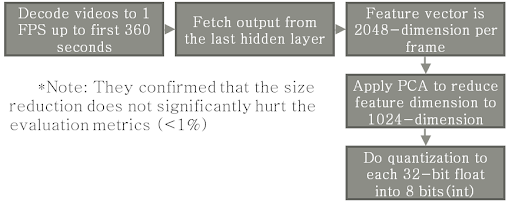
\includegraphics[width=1\textwidth]{chapter2/images/decrease_data.png}
		\caption{ขั้นตอนกระบวนการการลดขนาดของชุดข้อมูลให้สามารถใช้งานได้ง่ายยิ่งขึ้น}
    	\label{fig:decrease_data}
\end{figure}




\subsubsection*{2. การทดลองและวิเคราะห์ผล}
ในบทความ \footnote{YouTube-8M,https://arxiv.org/pdf/1609.08675.pdf} นั้นได้นำเสนอวิธีการในการจัดการข้อมูลซึ่งแบ่งเป็น 2 รูปแบบตามลักษณะของข้อมูลที่ใช้ และอัลกอริทึมหรือเทคนิคที่ใช้ในการสร้างโมเดล ดังนี้
\begin{enumerate}
	\setlength\itemsep{-0.25em}
	\item คุณลักษณะระดับเฟรม (Frame-level feature)
	\begin{enumerate}
		\setlength\itemsep{-0.25em}
		\item Frame-Level Models and Average Pooling
		\\ อันดับแรกเนื่องจากว่าชุดข้อมูลนี้ไม่มีการระบุหัวข้อในระดับเฟรม จึงใช้วิธีการนำหัวข้อในระดับวิดีโอ มากำหนดให้กับทุกๆเฟรมในวิดีโอแทน จากนั้นสุ่มเฟรมมา 20 เฟรมในแต่ละวิดีโอ ทำให้มีเฟรมถึง 120 ล้านเฟรม ซึ่งในแต่ละหัวข้อ $e$ ทำให้มี $(x_{i}, y_{i}^{e})$ 120 ล้านคู่ โดยที่ $x_{i} \epsilon  R^{1024}$ คือ คุณลักษณะที่ได้มาจาก hidden layer สุดท้ายก่อนจะเป็น fully connected และ $y_{i}^{e} \epsilon  0,1$ คือหัวข้อสำหรับหัวข้อ $e$ ของตัวอย่างที่ $i^{th}$ แล้วสร้างโมเดลทั้งหมด 4,800 โมเดลที่เป็นโมเดลแบบ one vs all classifier และเป็นอิสระต่อกันสำหรับแต่ละหัวข้อ และเนื่องจากการประเมินผลนั้นมีพื้นฐานมาจากหัวข้อในระดับวิดีโอ ทำให้ต้องทำการรวมความน่าจะเป็นของแต่ละหัวข้อในระดับเฟรมไปเป็นความน่าจะเป็นในระดับวิดีโอ โดยใช้การเฉลี่ยค่าความน่าจะเป็นทั้งหมดในหัวข้อนั้นๆ และใช้ average pooling เพื่อลดผลจากการตรวจจับความผิดปกติและความโดดเด่นของข้อมูลของแต่ละหัวข้อภายในวิดีโอ
		\clearpage
		\item Deep Bag of Frames (DBoF) Pooling
		\begin{figure}[!ht]
			\centering
			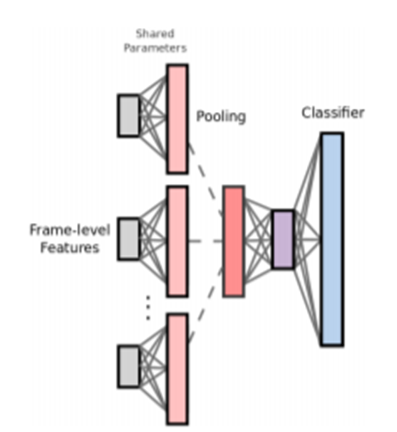
\includegraphics[width=0.5\textwidth]{chapter2/images/DBoF.png}
				\caption{โครงสร้างของโมเดล DBoF}
    			\label{fig:DBoF}
		\end{figure}
		\\ หลักการคล้ายๆกับ Deep Bag of Words โดยที่จะสุ่มเฟรม มา k เฟรม โดยที่แต่ละเฟรมเป็น N dimension input มาผ่าน fully connected ที่มี M units (M > N) และใช้ RELU activations แล้วทำ batch normalization ก่อนจะนำมารวมด้วย max pooling โดยที่ทั้งโครงข่ายใช้ Stochastic  Gradient Descent(SGD) 
		\item Long short-term memory(LSTM)
		\\ ในบทความ \footnote{YouTube-8M,https://arxiv.org/pdf/1609.08675.pdf} นี้ได้ใช้ LSTM แบบเดียวกับของ Beyond Short Snippets: Deep Networks for Video Classification \footnote{AVA,https://arxiv.org/pdf/1705.08421.pdf} แต่เนื่องจาก YouTube-8M นั้นผ่านการทำ preprocess มาแล้วทำให้ไม่สามารถใช้ raw video frame ได้ จึงทำได้เฉพาะ LSTM และ softmax layer เท่านั้น ตามรูปที่ \ref{fig:BSS}
		\begin{figure}[!ht]
			\centering
			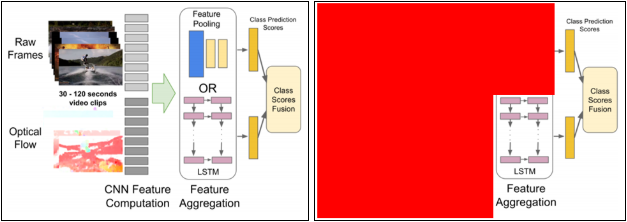
\includegraphics[width=1\textwidth]{chapter2/images/BSS.png}
				\caption{(ซ้าย) โครงสร้างจาก Beyond Short Snippets: Deep Networks for Video Classification, (ขวา) ส่วนที่สามารถใช้งานกับ YouTube-8M ได้}
    			\label{fig:BSS}
		\end{figure}
	\end{enumerate}
	\item คุณลักษณะระดับวิดีโอ (Video-level feature)
	\begin{enumerate}
		\setlength\itemsep{-0.25em}
		\item Video-level representation 
		\\ ในบทความ \footnote{YouTube-8M,https://arxiv.org/pdf/1609.08675.pdf}นี้ได้สำรวจวิธีการแยกเวกเตอร์คุณลักษณะระดับวิดีโอความยาวคงที่จากคุณลักษณะระดับเฟรมซึ่งการทำแบบนี้ทำให้ได้ประโยชน์ 3 ข้อ คือ 1) โมเดลทั่วไปที่ไม่ใช่ neural network สามารถนำไปใช้งานได้  2) ขนาดข้อมูลเล็กลง  3) เหมาะกับการนำไปสร้างโมเดล domain adaptive มากขึ้น
		\begin{enumerate}
			\setlength\itemsep{-0.25em}
			\item First, Second order and ordinal statistic
			\\ จากคุณลักษณะในระดับเฟรม $x_{1:F_{v}}^{v}$ โดยที่ $x_{j}^{v}$ คือคุณลักษณะระดับเฟรมในเฟรมที่ $j$ ของวิดีโอ $v$ และ $F_{v}$ คือจำนวนเฟรมทั้งหมดของวิดีโอ $v$ ทำการหาค่าเฉลี่ย $\mu_{v}$ และส่วนเบี่ยงเบนมาตรฐาน $\sigma_{v}$ พร้อมทั้งดึง ordinal statistics 5 อันดับแรกของแต่ละ dimension K ออกมา $Top_{k}(x^{v}(j)_{1:F_{v}})$ จะทำให้ได้เวคเตอร์คุณลักษณะ(feature-vector) $\varphi_{1:F_{v}}^{v}$ ของวิดีโอเป็นดังนี้ \\
			\centerline{$\varphi_{1:F_{v}}^{v} = \begin{bmatrix}
								\mu_{1:F_{v}}^{v}\\ 
								\sigma_{1:F_{v}}^{v}\\ 
								Top_{k}(x^{v}(j)_{1:F_{v}})
								\end{bmatrix}$}
			\item Feature normalization \\
			ก่อนที่จะทำการสร้าง one vs all classifiers แต่ละตัวนั้นได้ทำ normalization เวกเตอร์คุณลักษณะ $\varphi_{1:F_{v}}^{v}$ จากนั้นนำค่าเฉลี่ย $\mu_{v}$ ออกแล้วใช้ PCA ในการลด มิติของข้อมูล ซึ่งการทำแบบนี้นั้นทำให้การสร้างโมเดลเป็นไปได้เร็วขึ้น
		\end{enumerate}
		โดยการสร้างโมเดลด้วย video-level presentation นั้น บทความ \footnote{YouTube-8M,https://arxiv.org/pdf/1609.08675.pdf} นี้ได้หยิบมาทดสอบ 3 อัลกอริทึม
		\item Model training algorithm approaches 
		\begin{enumerate}
			\setlength\itemsep{-0.25em}
			\item Logistic Regression
			\item Hinge Loss
			\item Mixture of Experts (MoE)
		\end{enumerate}
		\item Evaluation metrics
		\begin{enumerate}
			\setlength\itemsep{-0.25em}
			\item Mean Average Precision (mAP)
			\item Hit@k
			\item Precision at equal recall rate (PERR)
		\end{enumerate}
	\end{enumerate}
	\item Results
	\begin{enumerate}
		\setlength\itemsep{-0.25em}
		\item Baseline on YouTube-8M dataset
\begin{table}[!ht]
\centering
\begin{tabular}{|c|c|c|c|c|}
		\hline
		{Inpute Features}&{Modeling Approach}&{mAP}&{Hit@1}&{(PERR)}\\
		\hline
		Frame-level, $(x_{1:F_{v}}^{v})$	& Logistic + Average		& 11.0		& 50.8		& 42.2					\\
		Frame-level, $(x_{1:F_{v}}^{v})$	& Deep Bag of Frames	& 26.9		& 62.7		& 55.1					\\
		Frame-level, $(x_{1:F_{v}}^{v})$	& LSTM				& 26.6		& 64.5		& 57.3					\\
		\hline
		Video-level, $\mu$					& Hinge loss					& 26.6		& 64.5		& 57.3				\\
		Video-level, $\mu$					& Logistic Regression				& 26.6		& 64.5		& 57.3				\\
		Video-level, $\mu$					& Mixture-of-2-Expert				& 26.6		& 64.5		& 57.3				\\
		Video-level, $\mu ; \sigma ; Top_{5} $	& Mixture-of-2-Expert				& 26.6		& 64.5		& 57.3				\\
		\hline
	\end{tabular}
	\caption{ประสิทธิภาพของโมเดลที่สร้างจาก YouTube-8M ด้วยวิธีต่างๆตามหัวข้อที่ 1 และ 2 โดยแถวที่ 1 คือ frame-level โมเดลและแถวที่ 2 คือ video-level โมเดล}
	\label{tab: ประสิทธิภาพของโมเดลที่สร้างจาก YouTube-8M}
\end{table}
\\
		จากตารางที่ \ref{tab: ประสิทธิภาพของโมเดลที่สร้างจาก YouTube-8M} จะเห็นว่าการทำ video-level features จากการหาค่าเฉลี่ยของ frame-level features แล้วสร้างโมเดลด้วย Hinge loss หรือ โมเดล Logistic Regression นั้นสามารถเพิ่มประสิทธิภาพได้ไม่น้อย และจากการทดลองทำให้เห็นว่า LSTM ที่มีความลึก 2 layers นั้นสามารถทำให้ผลลัพธ์เป็น state-of-the-art ในขณะนั้นได้ เนื่องจากในขณะที่ DBoF นั้นไม่ได้สนใจลำดับของเฟรม แต่ LSTM ใช้ state information เพื่อคงลำดับของเฟรมเอาไว้
\\
\\
		 LSTM นั้นดีที่สุดยกเว้น mAP, เนื่องจาก one-vs-all binary MoE classifier นั้นมีประสิทธิภาพดีกว่า, LSTM สามารถเพิ่มประสิทธิภาพบน Hit@1 และ PERR ได้เนื่องจากความสามารถในการเรียนรู้ความสัมพันธ์ระยะยาวในโดเมนของเวลา
		\clearpage
		\item Transfer learning video-level presentation from YouTube-8M to Sports-1M dataset
\begin{table}[!ht]
\centering
\begin{tabular}{|c|c|c|c|}
		\hline
		{Approach}&{mAP}&{Hit@1}&{(Hit@1)}\\
		\hline
		Logistic Regression ($\mu$)					& 58.0		& 60.1		& 79.6					\\
		Mixture-of-2-Expert ($\mu$)					& 59.1		& 61.5		& 80.4					\\
		Mixture-of-2-Expert ([$\mu ; \sigma ; Top_{5}$		& 61.3		& 63.2		& 82.6					\\
		LSTM									& 66.7		& 64.9		& 85.6					\\
		+Pretrained on YT-8M							& 67.6		& 65.7		& 86.2					\\
		\hline
		Hierarchical 3D Convolution						& -			& 61.0		& 80.0					\\
		Stacked 3D Convolutions						& -			& 61.0		& 85.0					\\
		LSTM with Optical Flow and Pixels				& -			& 73.0		& 91.0					\\
		\hline
	\end{tabular}
	\caption{ประสิทธิภาพของโมเดลเมื่อถูก transfer learning ด้วยชุดข้อมูล Sports-1M โดยใช้ video-level presentation}
	\label{tab: transfer learning}
\end{table}
\\
		จากตารางที่  \ref{tab: transfer learning} จะเห็นว่าโมเดล LSTM ที่ถูก pretrained จาก YouTube-8M นั้นมีประสิทธิภาพที่ดีกว่า ยกเว้น LSTM with Optical Flow and Pixels ที่มีการใช้ข้อมูลการเคลื่อนไหว(optical flow) ในการสร้างโมเดลด้วย
\\

		\item Transfer learning video-level presentation from YouTube-8M to ActivityNet dataset
\begin{table}[!ht]
\centering
\begin{tabular}{|c|c|c|c|}
		\hline
		{Approach}&{mAP}&{Hit@1}&{(Hit@1)}\\
		\hline
		Mixture-of-2-Expert ($\mu$)					& 69.1		& 68.7		& 85.4					\\
		+Pretrained PCA on YT-8M						& 74.1		& 72.5		& 89.3					\\
		Mixture-of-2-Expert ([$\mu ; \sigma ; Top_{5}$		& NO			& 74.2		& 72.3					\\
		+Pretrained PCA on YT-8M						& 77.6		& 74.9		& 91.6					\\
		LSTM									& 57.9		& 63.4		& 81.0					\\
		+Pretrained on YT-8M							& 75.6		& 74.2		& 92.4					\\
		\hline
		Ma, Bargal et al.								& 53.8		& -			& -						\\
		Heilbron et al.								& 43.0		& -			& -						\\
		\hline
	\end{tabular}
	\caption{ประสิทธิภาพของโมเดลเมื่อถูก transfer learning ด้วยชุดข้อมูล ActivityNet โดยใช้ video-level presentation}
	\label{tab: transfer learning ActivityNet}
\end{table}
\\
		จากตารางที่ \ref{tab: transfer learning ActivityNet} จะเห็นว่าโมเดลที่ถูก pretrained จาก YouTube-8M นั้นมีประสิทธิภาพที่ดีขึ้นมากเมื่อเทียบกับ benchmark ก่อนหน้า
	\end{enumerate}
\end{enumerate}

\subsubsection*{3. ปัญหาที่พบ}
เนื่องจากว่า YouTube-8M นั้นมีจำนวนข้อมูลที่เยอะมาก ทำให้ไม่สามารถตรวจสอบได้ทั้งหมดว่า ground-truth ของแต่ละวิดีโอนั้นมีความถูกต้องมากน้อยขนาดไหน ทำให้อาจเกิดข้อผิดพลาดได้ (ปัจจุบัน ปี 2019 YouTube-8M ได้มีการตรวจสอบข้อมูลอีกครั้ง เพื่อเพิ่มประสิทธิภาพของชุดข้อมูลซึ่งทำให้ปัจจุบันจำนวนข้อมูล และจำนวน category นั้นจะลดน้อยลงจากข้อมูลที่ใช้อ้างอิงในบทความ \footnote{YouTube-8M,https://arxiv.org/pdf/1609.08675.pdf} ข้างต้นที่ได้กล่าวมา)







%\clearpage
%AVA\textsuperscript{\cite{AVA}} คือ ชุดข้อมูลที่รวบรวมวิดิโอที่มีความยาว 15 นาที ถูกแบ่งด้วยความถี่ 1 hz (900 keyframes) จากในภาพยนต์โดยยึดการกระทำของมนุษย์เป็นศูนย์กลาง
เพื่อใช้สำหรับสร้างโมเดลที่เข้าใจกิจกรรมของมนุษย์ในวิดิโอว่ามนุษย์กำลังทำอะไรอยู่ ซึ่งข้อดีของ AVA คือ ชุดข้อมูลจะมีคำกำกับเป็นแบบทวิคำกำกับ (multiple label)
และคำกำกับของ AVA มีจำนวน 80 ประเภท สามารถแบ่งได้เป็นสามหมวดหมู่คือ ท่าทาง (Pose), ปฏิสัมพันธ์กับวัตถุ (Interaction with object) 
และปฏิสัมพันธ์กับบุคคล (Interaction with people) ซึ่งสามารถมีคำกำกับได้มากสูงสุดถึง 7 คำกำกับ
\begin{enumerate}
	\item {รายละเอียดชุดข้อมูล}
	\begin{enumerate}
		\item ขั้นตอนการเก็บข้อมูลสำหรับการทำชุดข้อมูลมีขั้นตอนการทำ 5 ขั้นดังนี้
		\begin{enumerate}
			\item การสร้างคำศัพท์การกระทำจะมีหลักการ 3 ข้อในการรวบรวมคำศัพท์ดังนี้
			\begin{enumerate}
				\item เก็บรวบรวมคำศัพท์ทั่วไปที่เกิดขึ้นในชีวิตประจำวัน
				\item จะต้องมีเอกลักษณ์สามารถเห็นได้ชัดเจน เช่น การถือของ
				\item กำหนดรูปแบบของคำศัพท์ขึ้นมา และใช้ความรู้จากชุดข้อมูลอื่นในการทำให้ได้หมวดหมู่การกระทำของมนุษย์ที่ครอบคลุม
			\end{enumerate}
			\item ภาพยนต์และส่วนที่เลือกมาใช้ทำชุดข้อมูล AVA ทั้งหมดจะถูกนำมาจาก YouTube โดยเริ่มจากการรวบรวมเอารายชื่อของนักแสดงที่มีชื่อเสียง
			ซึ่งจะมีความหลากหลายของเชื้อชาติรวมกันอยู่ วิดีโอที่ถูกคัดเลือกจะมีเกณฑ์ดังนี้
			\begin{enumerate}
				\item วิดีโอต้องอยู่ในหมวด ภาพยนต์ และละครโทรทัศน์
				\item วิดีโอจะต้องมีความยาวมากกว่า 30 นาที
				\item เผยแพร่มาแล้วเป็นระยะเวลาอย่างน้อย 1 ปี
				\item มีจำนวนยอดคนดูมากกว่า 1,000 ครั้ง
				\item ละเว้นวิดีโอบางประเภท เป็นภาพขาว-ดำ มีความละเอียดต่ำ การ์ตูน หรือวิดีโอเกม
			\end{enumerate}
			\item การสร้างกรอบสี่เหลี่ยมครอบมนุษย์ที่อยู่ภายในภาพประกอบด้วย 2 ขั้นตอน
			\begin{enumerate}
				\item สร้างกรอบสี่เหลี่ยมโดยใช้โมเดลปัญญาประดิษฐ์ faster RCNN สำหรับการตรวจจับมนุษย์
				\item ใช้มนุษย์ในการตรวจสอบและแก้ไขกรอบสี่เหลี่ยมที่ผิดพลาด
			\end{enumerate}	
			\item การติดตามตำแหน่งของบุคคล\\
			ทำการติดตามตำแหน่งของบุคคลที่อยู่ในช่วงเวลาเดียวกันด้วยใช้วิธีการแทร็กโดยยึดมนุษย์เป็นศูนย์กลาง โดยการคำนวณค่าความใกล้เคียงกันระหว่างบุคคล 
			โดยใช้ person embedding (ใช้โครงข่ายประสาทเทียมในการหาฟีเจอร์ขั้นสูงและใช้เมทริกซ์ในการหาความสัมพันธ์ของแต่ละคน) จากนั้นจะใช้อัลกอริทึม Hungarian distance (อัลกอริทึ่มสำหรับการหาข้อเสนอที่ดีที่สุด) ในการหาตัวเลือกคู่ของกรอบสี่เหลี่ยมที่ดีที่สุด
			\item การสร้างคำกำกับคุณลักษณะ\\
			การสร้างคำกำกับของการกระทำจะถูกสร้างขึ้นโดยมนุษย์ ซึ่งผู้วิจัยจะใช้โปรแกรมสำหรับช่วยเหลือในการสร้างคำกำกับคุณลักษณะ โดยสามารถกำหนดคำกำกับของการกระทำได้สูงสุดถึง 7 คำต่อ 1 กรอบสี่เหลี่ยม นอกจากนั้นสามารถตั้งสถานะเนื้อหาที่ไม่เหมาะสม หรือ กรอบสี่เหลี่ยมที่ผิดพลาดได้อีกด้วย ซึ่งในทางปฎิบัติเพื่อลดโอกาสที่จะเกิดข้อผิดพลาด จึงแบ่งขั้นตอนในการสร้างคำกำกับออกเป็น 2 ขั้นตอนดังนี้
			\begin{enumerate}
				\setlength\itemsep{-0.25em}
				\item สร้างข้อเสนอสำหรับคำกำกับของการกระทำ
				\item ข้อเสนอจะถูกตรวจสอบข้อเสนอที่ได้จากขั้นตอนแรก ซึ่งจะใช้มนุษย์ในการตรวจสอบ 3 คน โดยคำกำกับจะต้องถูกตรวจสอบด้วยผู้ตรวจสอบอย่างน้อย 2 คน จึงจะถูกยึดเป็นคำกำกับหลัก
			\end{enumerate}
		\end{enumerate}
	\end{enumerate}
	\item {โมเดลปัญญาประดิษฐ์}
	\begin{enumerate}
		\item โมเดลปัญญาประดิษฐ์ที่งานวิจัยนี้ใช้ คือ two stream variant ซึ่งจะทำการประมวลผลทั้ง RGB flow และ optical flow 
		โดยเป็นโครงสร้างของ faster RCNN ที่นำ Inception network เข้ามาใช้
		\item เครื่องมือที่ใช้วัดผลสำหรับงานวิจัยนี้ คือค่า IoU และ 3D IoUs 
		\begin{enumerate}
			\item ค่า IoU คือค่าที่ใช้วัดความสอดคล้องระหว่างสองกรอบสี่เหลี่ยม(กรอบสี่เหลี่ยมจริงของเฟรม และ กรอบสี่เหลี่ยมที่ทำนายขึ้นมา) ซึ่งใช้สำหรับการวัดผลระดับเฟรม 
			\item ค่า 3D IoUs คือค่าที่ใช้วัดความสอดคล้องระหว่างกรอบสี่เหลี่ยมภายใน 2 วิดีโอ ซึ่งใช้สำหรับการวัดผลระดับวิดีโอ โดยเทียบกันระหว่างกรอบสี่เหลี่ยมจริงในช่วงของเฟรมที่ต่อกัน (ground-truth tubes) และ กรอบสี่เหลี่ยมที่ทำนายขึ้นมาในช่วงของเฟรมที่ต่อกัน (linked detection tubes) 
		\end{enumerate}
		\item ประสิทธิภาพของโมเดลปัญญาประดิษฐ์ในปัจจุบัน
		\\ข้อมูลโมเดลปัญญาประดิษฐ์ที่นำมาทดสอบ
		\begin{enumerate}				
			\item Actionness\textsuperscript{\cite{actioness}} เป็นการหาความน่าจะเป็นของการกระทำ โดยใช้โครงสร้างของ hybrid fully convolutional network (HFCN) hybrid fully เป็นโครงสร้างที่ประกอบด้วยโครงข่ายประสาทเทียม 2 ชนิด คือ
			\begin{enumerate}
				\item Appearance-FCN (A-FCN) คือ โครงข่ายประสาทเทียมที่นำมาใช้แสดงลักษณะของวัตถุ(ตำแหน่งวัตถุ, ความตื้นลึกวัตถุ) ที่ปรากฎบนรูป RGB1
				\item MotionFCN (M-FCN) คือ โครงข่ายประสาทเทียมที่แยกการเคลื่อนไหวจากข้อมูลของ optical flow
			 \end{enumerate}
			\item Peng without MR, Peng with MR (Multi-region two-stream R-CNN)\textsuperscript{\cite{peng}} เป็นโมเดลปัญญาประดิษฐ์ที่ใช้สำหรับตรวจจับวิดีโอในชีวิตจริง ซึ่งพื้นฐานของโมเดลนี้เป็น Faster R-CNN โดยโมเดลนี้มีกระบวนการ 3 กระบวนการคือ
			\begin{enumerate}
					\item สร้างข้อเสนอพื้นที่ที่มีการเคลื่อนไหว
					\item สะสม Optical flow จากเฟรมหลายๆเฟรม เพื่อนำไปปรับปรุงการตรวจจับการกระทำ
					\item นำพื้นที่หลายๆส่วนมาวิเคราะห์ผ่านโมเดล Faster R-CNN
			\end{enumerate}
			\item ACT Action Tubelet Detector\textsuperscript{\cite{act}} เป็นการระบุตำแหน่งของการกระทำที่มีระยะเวลาๆสั้นๆ ซึ่งใช้วิธีการตรวจจับระดับเฟรม และ ใช้การติดตามตำแหน่งในการเชื่อมระหว่างเฟรมปัจจุบันไปยังเฟรมถัดไป. ACT ถูกสร้างต่อจาก SSD framework และ ใช้คอนโวลูชันในการสกัดคุณลักษณะในแต่ละเฟรมซึ่งการคิดคะแนนและความน่าจะเป็นของหมวดหมู่จะคิดจากการนำคุณลักษณะเรียงต่อกัน และ หาข้อมูลจากลำดับข้อมูลนั้น
		\end{enumerate}
		จากการทดสอบการเทียบโมเดลปัญญาประดิษฐ์ของงานวิจัยนี้และวิธีการอื่นๆ โดยนำไปทดสอบกับชุดข้อมูลวิดีโอ JHMDB และ UCF101-24 ได้ผลลัพธ์ออกมาดังนี้
			\begin{table}[!ht]
				\centering
				\begin{tabular}{|c|c|c|c|}
					\hline
					{Frame-mAP}&{JHMDB (mAP)}&{UCF101-24 (mAP)}								\\
					\hline
					Actionness 			& 39.9				& 	-						\\
					Peng w/o MR			& 56.9				& 64.8						\\
					Peng w/  MR 			& 58.5				& 65.7						\\
					ACT					& 65.7				& 69.5						\\
					\hline
					2 stream(Our approach)		& \textbf{73.3}		& \textbf{76.3}				\\
					\hline
				\end{tabular}
				\caption{ผลการทดลองของวิธีต่างๆบนคุณลักษณะระดับเฟรม}
				\label{tab: transfer learning}
			\end{table}
		\item ปัญหาที่พบ
		ในปัจจุบันยังไม่มีโมเดลปัญญาประดิษฐ์ที่ทดสอบด้วยชุดข้อมูล AVA และได้ผลการทำงานที่ดี เนื่องจากชุดข้อมูลนี้สนใจการกระทำของมนุษย์ที่มีรายละเอียดเล็กๆน้อยๆ 
		ทำให้ยากต่อการทำนายสำหรับโมเดลปัญญาประดิษฐ์
	\end{enumerate}
\end{enumerate}
%\clearpage
%Moments in time\textsuperscript{\cite{monfort2019moments}} คือชุดข้อมูลที่ใช้มนุษย์ในการกำกับข้อมูลทั้งหมดให้กับวิดีโอสั้นถึง 1 ล้านวิดีโอ 
และมีจำนวนกิจกรรมหรือการกระทำต่างกัน 339 หมวดหมู่ โดยแต่ละวิดีโอจะมีความยาวอยู่ที่ 3 วินาที เนื่องจากเป็นเวลาเฉลี่ยที่มนุษย์ใช้ในการเข้าใจกับเหตุการณ์ที่เกิดขึ้น
(human working memory) รูปแบบของชุดข้อมูลจะมีอยู่ทั้งหมดอยู่ 3 รูปแบบ ได้แก่ ภาพนิ่ง (spatial) เสียง (auditory) และการเคลื่อนไหว (temporal) 
นอกจากนี้ชุดข้อมูลนี้นั้นไม่รวบรวมเพียงแค่การกระทำของมนุษย์เท่านั้น ยังรวมไปถึง สัตว์ สิ่งของ และปรากฏการณ์ธรรมชาติ ทำให้ชุดข้อมูลนี่เป็นการท้าทายรูปแบบใหม่เพราะด้วยข้อมูลที่มีความซับซ้อนมากขึ้น
\begin{enumerate}
	\item {รายละเอียดชุดข้อมูล}
	\begin{enumerate}
		\setlength\itemsep{-0.25em}
		\item เป้าหมายของชุดข้อมูล : สนใจเหตุการณ์ที่เกิดขึ้นในวิดีโอ เช่น การกระทำของคนหรือสัตว์ เหตุการณ์ และปรากฎการณ์ธรรมชาติ 
		\item จำนวนของวิดีโอ : มากกว่า 1,000,000 วิดีโอ
		\item ความยาวเฉลี่ยของแต่ละวิดีโอ : 3 วินาที
		\item จำนวนของหมวดหมู่ : 339 หมวดหมู่
		\item วิธีการเก็บรวบรวมข้อมูล
	\begin{enumerate}
		\item เริ่มจากการรวบรวมคำที่ใช้อยู่ทั่วไปในชีวิตประจำวันมา 4,500 คำจาก VerbNet\textsuperscript{\cite{Schuler:2005:VBC:1104493}} เว็บไซต์ที่เก็บรวบรวมคำกิริยาภาษาอังกฤษขนาดใหญ่ 
		จากนั้นนำมาแบ่งกลุ่มคำที่มีความหมายใกล้เคียงกันโดยใช้คุณลักษณะจาก Propbank\textsuperscript{\cite{Zaghouani:2010:RAP:1868720.1868756}} และ
		FrameNet\textsuperscript{\cite{Baker:1998:BFP:980451.980860}} โดยเก็บข้อมูลเป็นแบบเวกเตอร์คุณลักษณะฐานสอง (binary feature vector) 
		ซึ่งถ้าคำใดมีความเกี่ยวข้องกันทางคุณลักษณะก็จะให้ค่าเป็น 1 ถ้าไม่เกี่ยวข้องกันจะให้ค่าเป็น 0 จากนั้นจึงใช้วิธี k-means clustering ในการแบ่งกลุ่ม 
		เมื่อแบ่งกลุ่มแล้วจากนั้นจะเลือกคำจากในแต่ละกลุ่มนั้น โดยคำที่เลือกมานั้นจะเป็นคำที่ใช้บ่อยที่สุดในกลุ่มนั้น และลบคำนั้นออกจากกลุ่มอื่นๆทั้งหมด (คำๆหนึ่งสามารถอยู่ได้หลายกลุ่ม) 
		จากนั้นจะทำกระบวนการนี่ไปเรื่อยๆ แต่คำที่เลือกมาจะต้องไม่มีความหมายคลุมเครือ หรือเป็นสิ่งที่ไม่สามารถมองเห็นหรือได้ยินได้ และต้องไม่มีความหมายเหมือนกับคำที่เคยเลือกมาก่อน 
		จนสุดท้ายแล้วได้ออกมาที่ 339 หมวดหมู่
		\item ต่อมาทำการหาชุดข้อมูลวิดีโอโดยจะตัดออกมาเพียง 3 วินาทีที่เกี่ยวข้องกับคำใน 339 หมวดหมู่ที่เลือกมาจากวิดีโอแหล่งต่างกัน 10 แหล่ง 
		การตัดวิดีโอนั้นจะไม่ใช้พวก Video2Gif (โมเดลที่ระบุตำแหน่งของสิ่งที่น่าสนใจในวิดีโอ) เพราะจะทำให้เกิดอคติขึ้นจะเกิดขึ้นตอนสร้างโมเดล ดังนั้นจึงใช้มนุษย์ในการตัดวิดีโอ จากนั้นจะทำการส่งข้อมูลของคำ
		และวิดีโอที่ตัดไปยัง Amazon Mechanical Turk (AMT หรือตลาดแรงงาน) เพื่อทำการสร้างคำกำกับโดยพนักงานของ AMT ทำให้ได้ 64 วิดีโอที่เกี่ยวข้องกับคำหนึ่ง 
		และอีก 10 วิดีโอที่มีคำกำกับอยู่แล้ว โดยวิดีโอที่มีคำกำกับอยู่แล้วนั้นถ้าพนักงานของ AMT ตอบเหมือนกันเกิน 90\% ถึงจะนำเข้าไปรวมกับชุดข้อมูลส่วนอีก 64 วิดีโอ
		ถ้าเป็นชุดข้อมูลสำหรับสร้างโมเดลจะต้องผ่านพนักงานของ AMT อย่างน้อย 3 ครั้ง และต้องมีคำกำกับเหมือนกัน 75\% ขึ้นไปถึงจะถือว่าเป็นคำกำกับที่ถูกต้อง 
		ถ้าเป็นชุดข้อมูลสำหรับตรวจคำตอบ และชุดข้อมูลสำหรับทดสอบจะต้องผ่านพนักงานของ AMT อย่างน้อย 4 ครั้ง และต้องมีคำกำกับเหมือนกัน 85\% ขึ้นไป 
		เหตุผลที่ไม่ตั้งเกณฑ์ไว้ที่ 100\% เพราะจะทำให้วิดีโอนั้นยากเกินไปที่จะทำให้สามารถจำการกระทำได้	
	\end{enumerate}
\end{enumerate}
	\item การเตรียมข้อมูล
		\begin{enumerate}
			\item ชุดข้อมูลสำหรับสร้างโมเดลจะมี 802,264 วิดีโอ และมีวิดีโอในแต่ละหมวดหมู่อยู่ที่ 500 ถึง 5,000 วิดีโอ
			\item ชุดข้อมูลสำหรับตรวจคำตอบจะมี 33,900 วิดีโอ และมีวิดีโอในแต่ละหมวดหมู่อยู่ที่ 100 วิดีโอ
			\item แยกเฟรม RGB ออกมาจากวิดีโอ และทำการเปลี่ยนขนาดให้เป็น 340\texttimes256  pixel
			\item ใช้อัลกอริทึม TVL1 optical flow จาก Opencv เพื่อลดข้อมูลรบกวนที่จะเกิดขึ้น
			\item ทำการแปลงค่าที่อยู่ใน optical flow ให้เป็นเลขจำนวนเต็มเพื่อทำให้การคำนวณนั้นเร็วยิ่งขึ้น
			\item ปรับค่า displacement ใน optical flow ให้ค่าสูงสุดเป็น 15 ต่ำสุดเป็น 0 และทำการปรับขนาดให้เป็นช่วง 0 - 255
			\item เก็บข้อมูลออกมาในรูปแบบของภาพขาวดำเพื่อลดพื้นที่ในการเก็บข้อมูล
			\item แก้ปัญหาเรื่องการเคลื่อนไหวของกล้องด้วยการนำค่าเฉลี่ยของเวกเตอร์ไปลบกับ displacement
			\item สุดท้ายจะเป็นสุ่มตัดภาพออกมาเพื่อเพิ่มจำนวนข้อมูล
		\end{enumerate}
	\item {โมเดลปัญญาประดิษฐ์}
	\begin{enumerate}
		\item ในงานวิจัยนี้มีการทดสอบโมเดลปัญญาประดิษฐ์หลายรูปแบบ โดยโมเดลปัญญาประดิษฐ์ที่มีประสิทธิภาพการทำงานที่ดีที่สุด 5 ลำดับแรกมีดังนี้
			\begin{enumerate}
				\item SVM มีรูปแบบข้อมูลที่ป้อนเข้า คือ เฟรมที่ต่อเนื่อง (spatial) + เฟรมเดี่ยว (temporal) + ข้อมูลเสียง (auditory) 	
				\item I3D มีรูปแบบข้อมูลที่ป้อนเข้า คือ เฟรมที่ต่อเนื่อง + เฟรมเดี่ยว
				\item TRN-Multiscale มีรูปแบบข้อมูลป้อนเข้า คือ เฟรมที่ต่อเนื่อง + เฟรมเดี่ยว
				\item TSN-2stream มีรูปแบบข้อมูลป้อนเข้า คือ เฟรมที่ต่อเนื่อง + เฟรมเดี่ยว
				\item ResNet50-ImageNet	มีรูปแบบข้อมูลป้อนเข้า คือ เฟรมที่ต่อเนื่อง
			\end{enumerate}
		\item เครื่องมือที่ใช้วัดผลงานวิจัยนี้
			\begin{enumerate}
				\item Classification accuracy Top-1, Top-5
			\end{enumerate}
		\item ประสิทธิภาพของโมเดลปัญญาประดิษฐ์ในปัจจุบัน
			\begin{enumerate}
				\item ทำการทดสอบด้วยวิธี cross dataset transfer โดยการนำโมเดล ResNet50 I3D ที่สร้างด้วยชุดข้อมูล Kinetics และ Moments in Time 
				แล้วนำทั้ง 2 โมเดลไปทดสอบกับชุดข้อมูลอื่น โดยจะปรับอัตราความถี่ของเฟรม (frame rate) ของวิดีโอให้เป็น 5 fps
				\begin{table}[!ht]
					\centering
					\begin{tabular}{|c|c|c|c|}
						\hline
						{Pretrained}&\multicolumn{3}{c|}{Fine-Tuned}\\
						\cline{2-4}
						{}								& UCF-101			& HMDB-51			& Something Something			\\
						\hline
						\multirow{2}{*}{Kinetics}		& Top-1 : 92.6		& Top-1 : 62.0		& Top-1 : 48.6		\\
						{}								& Top-5 : 99.2		& Top-5 : 88.2		& Top-5 : 77.9		\\
						\hline
						\multirow{2}{*}{Moments}		& Top-1 : 91.9		& Top-1 : 65.9		& Top-1 : 50.0		\\
						{}								& Top-5 : 98.6		& Top-5 : 89.3		& Top-5 : 78.8		\\
						\hline
					\end{tabular}
					\caption{ประสิทธิภาพของโมเดล Resnet50 I3D ที่ใช้ชุดข้อมูล Kinetics และ Moments in Time}
					\label{tab: Data transfer performance ของโมเดล Resnet50 I3D}
				\end{table}
				\item จะเห็นได้ว่า Kinetics ให้ผลลัพธ์ที่ดีกว่าใน UCF-101 เพราะว่ามีหมวดหมู่ที่ตรงกันอยู่หลายอย่าง ในขณะที่ HMDB-51 นั้นมีการรวบรวมข้อมูลจากหลายแหล่ง 
				และมีจำนวนหมวดหมู่ที่หลากหลายจึงทำให้มีความใกล้เคียงกับตัวข้อมูลของ Moments in Time ดังนั้นจึงเทียบผลลัพท์จาก Something Something 
				ซึ่งจะทำให้เห็นว่า Moments in Time มีประสิทธิภาพที่ดีกว่าและวิดีโอที่มีความยาวมากกว่า 3 วินาทีจะไม่ส่งผลกระทบกับประสิทธิภาพของ Moments in Time
		\end{enumerate}
	\end{enumerate}
	\item {ปัญหาที่พบ}\\
	ผลลัพธ์จากการทำนายด้วยโมเดลถ้าผ่านภาพที่มีรายละเอียดเยอะจะทำให้การ ทำนายโอกาสผิดนั้นค่อนข้างสูง ซึ่งปัญหานี่สามารถทำให้เกิดน้อยลงด้วยการนำวิธี 
	class activation mapping (CAM) จะเป็นการเน้นภาพในส่วนที่มีข้อมูลมากที่สุดและทำนายผลออกมา แต่ก็ยังมีจุดที่เป็นปัญหาอยู่ เช่น 
	การกระทำที่เกิดขึ้นเร็วมากจะทำให้การทำนายนั้นมีโอกาสผิดสูงขึ้น
\end{enumerate}		

\section{ทฤษฎีที่เกี่ยวข้อง}
\subsection{Optical flow}
Optical flow \footnote{Optical flow,shorturl.at/mrtEZ}  คือรูปแบบของการเคลื่อนที่ของวัตถุในรูปภาพระหว่างภาพซึ่งอาจจะการจากเคลื่อน ที่ของวัตถุหรือตัวกล้อง ออกมาในรูปแบบของ เวกเตอร์(vector) 2 มิติ โดยที่เวกเตอร์แต่ละตัวจะแสดงถึงทิศทางการเคลื่อนที่ระหว่างภาพดังรูปด้านล่าง

\begin{figure}[!ht]
	\centering
	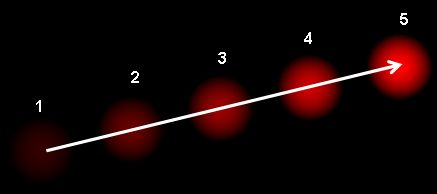
\includegraphics[width=1\textwidth]{chapter2/images/vector_optical.png}
		\caption{ตัวอย่างการเคลื่อนที่ของลูกบอล}
    	\label{fig:vector_optical}
\end{figure}

จากรูปภาพจะแสดงให้เห็นถึงการเคลื่อนที่ของลูกบอลของภาพที่ต่อเนื่องกัน 5 ภาพโดยที่ลูกศรแสดงถึงทิศทางการเคลื่อนที่ของเวกเตอร์
\\
\clearpage
\par
การทำงานของ optical flow อยู่บนสมมติฐานหลายประการได้แก่
\begin{enumerate}
	\setlength\itemsep{-0.25em}
	\item ความเข้มของพิกเซล(pixel) ของวัตถุจะไม่เปลี่ยนแปลงระหว่างภาพที่ต่อเนื่องกัน
	\item พิกเซลที่อยู่ใกล้กันจะมีการเคลื่อนไหวที่คล้ายกัน
\end{enumerate}

เมื่อพิจารณาพิกเซล I(x,y,t) จากภาพแรกจะเคลื่อนไหวเป็นระยะทาง (dx,dy) ไปยังภาพต่อไปหลังจากผ่านไปแล้ว dt เวลา ดังนั้นเนื่องจาก พิกเซล เหล่านี้เหมือนกันและความเข้มไม่มีการเปลี่ยนแปลง จึงทำให้พูดได้ว่า
\\
\centerline{$I(x,y,t) = I(x + dx, y + dy, t + dt)$}		\\
\centerline{$I$ คือ พิกเซลจากภายในภาพ}			\\
\centerline{$x$ คือ ตำแหน่งของพิกเซล ในแกน x} 		\\
\centerline{$dx$ คือ ระยะทางที่เคลื่อนที่ในแกน x} 		\\
\centerline{$y$ คือตำแหน่งของพิกเซลในแกน y} 		\\
\centerline{$dy$ คือ ระยะทางที่เคลื่อนที่ในแกน y}		\\
\centerline{$t$ คือ เวลา}						\\
\centerline{$dt$ คือ ระยะเวลาที่เปลี่ยนไประหว่างภาพ} 	\\

จากนั้นใช้การประมาณค่าของ taylor series ทางฝั่งขวามือและ ลบค่า common term และหารด้วย dt เพื่อให้ได้สมการดังต่อไปนี้
\\
\centerline{$f_{x}u + f_{y}v + f_{t} $}				\\
โดยที่
\\
\centerline{$f_{x} = \frac{\delta f}{\delta x} ; f_{y} = \frac{\delta f}{\delta y}$} 	\\
\centerline{$u = \frac{\delta x}{\delta t} ; v = \frac{\delta y}{\delta t}$}	 	\\
\centerline{$f_{x}$ คือ เกรเดียน(gradient) ในแกน x} 		\\
\centerline{$f_{y}$ คือ เกรเดียนในแกน y} 		\\
\centerline{$f_{y}$ คือ เกรเดียนของเวลา} 		\\
\centerline{$u$ คือ เวกเตอร์การเคลื่อนที่ของแกน x} 	\\
\centerline{$v$ คือ เวกเตอร์การเคลื่อนที่ของแกน y} 	\\

สมการข้างบนนี้จะเรียกว่าสมการ optical flow จากสมการทำให้สามารถหา $f_{x}$ และ $f_{y}$ โดยเป็น เกรเดียนของภาพ และ  $f_{t}$ เป็นเกรเดียน(gradient)ของเวลา แต่ $u$ กับ $v$ เป็นตัวแปรที่ไม่ทราบ ทำให้สมการนี้ไม่สามารถแก้ไขโดยมีตัวแปรที่ไม่ทราบถึง 2 ตัว จึงมีการนำวิธีการต่าง ๆ เข้ามาใช้ในการแก้ปัญหานี้ เช่น dense optical flow ซึ่งใช้อัลกอริทึมของ Gunner Farneback ซึ่งจะใช้วิธีการขยายพหุนาม\footnote{polynomial expansionfile:http://www.diva-portal.org/smash/get/diva2:273847/FULLTEXT01.pdf} (polynomial expansion)



\clearpage
\section{Two-Steam CNN}
\begin{figure}[!ht]
	\centering
	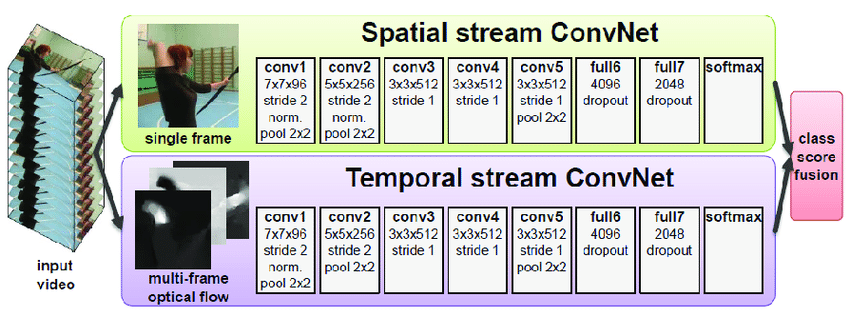
\includegraphics[width=1\textwidth]{chapter2/images/2steamCNN.png}
		\caption{แสดงโครงสร้างการทำงานของ two stream}
    	\label{fig:/2steamCNN}
\end{figure}

Two-Steam CNN \footnote{2steamCNN,https://papers.nips.cc/paper/5353-two-stream-convolutional-networks-for-action-recognition-in-videos.pdf} 
เป็นวิธีการหนึ่งในการทำ video classification โดยจะแบ่งออกเป็นสองกระบวนการทำไปพร้อมกัน คือ 
กระบวนการแรกนำรูปภาพเดี่ยวๆ มาใช้ซึ่งจะทำให้ได้ข้อมูลจากรูปภาพคือ ฉากและวัตถุต่างๆ และ 
กระบวนการที่สองนำลำดับของรูปภาพมาเพื่อดูการเคลื่อนไหวของวัตถุ 
และสุดท้ายจะนำข้อมูลที่ได้จากทั้งสองกระบวนการมารวมกันโดยใช้การ 
averaging หรือนำไปผ่าน linear SVM 





